\chapter{Theoretischer Hintergrund}

\section{Notation}

Die hier aufgeführte Notation orientiert sich zum Großteil an der Notation in \cite{kieffer_grammar-based_2000}:
\begin{itemize}
	\item $|\Sigma|$ beschreibt für eine endliche Menge $\Sigma$ die Anzahl der Elemente in $\Sigma$
	\item $|x|$ beschreibt für einen endlichen String $x$ die Länge von $x$
	\item $\Sigma^*$ bezeichnet die Menge aller Strings, deren einzelne Symbole Elemente aus $\Sigma$ sind. Also gilt für $x_0, \dots, x_{n-1} \in \Sigma$, dass $x_0 x_1 \dots x_{n-1} \in \Sigma^*$. Außerdem liegt auch der leere String $\varepsilon$ in $\Sigma^*$
	\item Für Strings $x, y \in \Sigma^*$ mit $|x| = n$ und $|y| = k$ ist $xy \in \Sigma^*$ definiert als die Konkatenation von $x$ und $y$, also $xy = x_0 \dots x_{n-1} y_1 \dots y_{k-1}$ 
	\item Sei $x = x_0 x_1 \dots x_{n-1} \in \Sigma^*$ ein String. Für $i \leq j$ ist dann $x[i..j]$ definiert als $x_i x_{i+1} \dots x_j \in \Sigma^*$ und heißt Substring von $x$. Ein Substring $P_i := x[0..i]$ heißt für $0 \leq i < n$ $i$-ter Präfix von $x$ und ein Substring $S_i := x[i..n - 1]$ heißt für $0 \leq i < n$ $i$-tes Suffix von $x$.
\end{itemize}

\section{Verlustfreie Datenkompression}

Datenkompression ist die Kodierung von Informationen in einer Repräsentation, die weniger Bits als die Eingabe benötigt \cite{mahdi_implementing_2012}. 
Im Gegensatz zur verlustbehafteten Kompression, die Daten komprimiert, indem nur geringfügig wichtige Information aus der Eingabe entfernt wird, lässt sich bei verlustfreier Kompression die gesamte Eingabe aus der komprimierten Repräsentation wiederherstellen. 

Dabei ist die Kompressionsrate definiert als das Verhältnis von der Länge des komprimierten Strings zur Länge des Eingabestrings.

\section{Straight-Line-Grammatiken}

Eine kontextfreie Grammatik $G = (N, \Sigma, P, S)$ ist ein 4-Tupel mit Nichtterminalsymbolen $N$, Terminalsymbolen $\Sigma$, $N \cap \Sigma = \emptyset$ und einem Startsymbol $S \in N$.
Die Grammatik enthält Produktionsregeln $P$ der Form $A \rightarrow \alpha$, mit $A \in N$ und $\alpha \in (N \cup \Sigma)^*$.

Wir schreiben 
\begin{equation*}
	\alpha B \gamma \Rightarrow \alpha \beta \gamma
\end{equation*}
für $\alpha, \beta, \gamma \in (N \cup \Sigma)^*$ und $B \in N$, falls eine Produktion $B \rightarrow \beta$ in $P$ existiert. 

Für $\alpha_i \in (N \cup \Sigma)^*, i = 0 \dots n, n \geq 1$ schreiben wir dann 
\begin{equation*}
	\alpha_0 \xRightarrow{n} \alpha_n
\end{equation*}
falls $\alpha_0 \Rightarrow \alpha_1, \alpha_1 \Rightarrow \alpha_2, \dots, \alpha_{n-1} \Rightarrow \alpha_n$ gelten. Das heißt also, dass sich $a_n$ aus $a_0$ durch Anwenden von $n$ Produktionsregeln aus $P$ ableiten lässt.
Falls es zu $\alpha, \beta \in (N \cup T)^*$ ein $n \in \mathbb{N}$ gibt, sodass $\alpha \xRightarrow{n} \beta$ gilt, dann schreiben wir 
\begin{equation*}
	\alpha \xRightarrow{*} \beta
\end{equation*}
Die Sprache von $G$ ist dann definiert als $L(G) := \{x \in \Sigma^*\ |\ S \xRightarrow{*} x\}$.

$G$ heißt nun Straight-Line-Grammatik, falls $|L(G)| = 1$, also die Grammatik genau ein Wort erzeugt. Die Grammatik hat somit weder Verzweigungen noch Schleifen \cite{benz_effective_2013}. 

\section{Grammatikbasierte Kompression}

Das Ziel der grammatikbasierten Kompression ist es, zu einem Eingabestring 
\begin{equation*}
	x = x_0 \dots x_{n-1} \in \Sigma^*
\end{equation*}
für ein Alphabet $\Sigma$, eine Straight-Line-Grammatik $G$ zu erzeugen, für die $L(G) = \{x\}$ gilt. Dabei sollte $G$ möglichst klein sein. 

Dazu in Verbindung steht das Problem, die kleinste Straight-Line-Grammatik zu einem String zu finden \cite{charikar_smallest_2005}. 
Dieses Problem ist allerdings $\mathcal{NP}$-vollständig \cite{charikar_smallest_2005}. Es ist nun also die Aufgabe, eine möglichst gute Approximation zu finden.
Die Größe einer Grammatik sei dabei definiert als die Summe der Länge aller rechten Seiten von Produktionsregeln in $P$ \cite{charikar_smallest_2005}, also:

\begin{equation*}
	|G| := \sum_{(A \rightarrow \alpha) \in P} |\alpha|
\end{equation*}

Die grundlegende Idee ist, für wiederholte Vorkommen von Substrings $x[i..j]$ in $x$ eine Produktion $A \rightarrow x[i..j]$ zu erzeugen und alle Vorkommen dieses Substrings durch das neue Nichtterminal $A \notin \Sigma$ zu ersetzen.

Es gibt Online-Algorithmen \cite{dinklage_compression_2017}, die die Eingabe von links nach rechts einlesen und schrittweise während des Lesens eine Grammatik aufbauen und anpassen. Ein Vertreter von Online-Algorithmen ist etwa Sequitur \cite{nevill-manning_identifying_1997}. 
Andererseits gibt es Offline-Algorithmen \cite{dinklage_compression_2017}, die die gesamte Eingabe in den Speicher laden und ganz betrachten um zu ersetzende Substrings auszuwählen. Ein Beispiel wäre Re-Pair \cite{larsson_offline_1999}.

Mit Methoden, eine möglichst kleine Grammatik zu erzeugen, wurde sich bereits beschäftigt \cite{benz_effective_2013, carrascosa_choosing_2010, charikar_smallest_2005}. 

\section{Enhanced Suffix-Array}

Das Enhanced Suffix-Array \cite{abouelhoda_replacing_2004} beschreibt im Allgemeinen das Suffix-Array \cite{manber_suffix_1993}, das mit verschiedenen anderen Tabellen, die im Folgenden beschrieben werden, ausgestattet wurde.

Es sei nun $x = x_0 x_1 \dots x_{n-1}\in \Sigma^*$ ein String mit $|x| = n$ über dem Alphabet $\Sigma$ 

\subsection{Suffix-Array}

Das Suffix-Array ist ein Array $SA$ mit $n$ Indizes $0 \leq i < n$, so dass 
\begin{equation*}
	S_{SA[0]}, S_{SA[1]}, \dots, S_{SA[n-1]}
\end{equation*}
die lexikographisch sortierte Reihenfolge der Suffixe des String $x$ ist \cite{abouelhoda_replacing_2004, manber_suffix_1993}.

Ein Eintrag $SA[i]$ beschreibt also den Index in $x$, an dem das lexikographisch $i$-kleinste (bei $0$ anfangend) Suffix beginnt. $SA$ kann in Laufzeit $\mathcal{O}(n)$ berechnet werden \cite{nong_two_2011}. 

Oftmals wird an $x$ noch ein weiteres Symbol $\$ \notin \Sigma$ angehängt, das lexikographisch kleiner (etwa \cite{fischer_inducing_2011, nong_two_2011}) oder größer (etwa \cite{abouelhoda_optimal_2002}) als alle Zeichen in $x$ ist. Für den String $x\$ = x_0\dots x_{n-1} \$$ und das zugehörige Suffix-Array gilt dann: $SA[0] = n$ und $S_{SA[0]} = \$$ beziehungsweise $SA[n] = n$ und $S_{SA[n]} = \$$. 
Dieses Suffix repräsentiert dann das leere Suffix. In dieser Arbeit wird $\$$ als lexikographisch \textit{größer} gewählt.

\subsection{Inverses Suffix-Array}

Das Inverse Suffix-Array zu einem Suffix-Array $SA$ ist ein Array $ISA$ mit $n$ Indizes \\
$0 \leq i < n$ so dass $SA[ISA[i]] = i$.
Ein Eintrag $ISA[i]$ beschreibt also den Suffix-Array Index des Suffixes $S_i$ von $x$.

$ISA$ kann trivial in Laufzeit $\mathcal{O}(n)$ nach der obigen Vorschrift berechnet werden \cite{abouelhoda_replacing_2004}.

\subsection{LCP-Array}

Das LCP-Array ist ein Array $LCP$, für das zu einem gegebenen Suffix-Array $SA$ gilt: 

Es sei $LCP[0] := 0$. Es gilt $LCP[i] = k$ für $1 \leq i < n$ wenn der längste gemeinsame Präfix von $S_{SA[i-1]}$ und $S_{SA[i]}$ die Länge $k$ hat. $LCP[i]$ ist also die Länge des längsten gemeinsamen Präfixes zweier lexikographisch benachbarter Suffixe von $x$. 

Das LCP-Array kann mithilfe von $SA$ \cite{kasai_linear-time_2001} oder alternativ während der Berechnung von SA \cite{fischer_inducing_2011} in $\mathcal{O}(n)$ Laufzeit berechnet werden.

\section{Predecessor Datenstrukturen}

\subsection{Predecessor-Problem}

Nach \cite{dinklage_engineering_2021} ist das Predecessor-Problem die Aufgabe, eine Menge $S \subset \mathbb{Z}$ zu verwalten, sodass folgende Operationen für ein $x \in \mathbb{Z}$ möglich sind:

\begin{itemize}
	\item $\texttt{insert(x)}$ Einfügen von $x$ in die Datenstruktur
	\item $\texttt{delete(x)}$ Löschen von $x$ aus der Datenstruktur
	\item $\texttt{predecessor(x)}$ Abfrage des größten $x' \in S$ mit $x' \leq x$
\end{itemize}

Eine Predecessor-Datenstruktur ist dann eine Datenstruktur, die das Predecessor-Problem möglichst effizient löst.

\subsection{Bucket-Predecessor-Struktur}

In der finalen Version des in dieser Arbeit vorgestellten Algorithmus kommt eine Version der Predecessor-Datenstruktur aus Kapitel 4 in \cite{dinklage_engineering_2021} zum Einsatz.

Diese basiert darauf, ein Universum $U$ der Größe $u := |U|$, in Buckets der Größe $b \ll u$ eingeteilt werden. Dabei ist $b = 2^k$ für ein $k \in \mathbb{N}$. Für ein $i \in \{0, \dots, u \backslash b \}$ erhält dann der Bucket an Index $i$ nur Schlüssel im Interval $[bi, b(i + 1) - 1]$. Ein Bucket heißt \textit{aktiv}, wenn er mindestens einen Schlüssel aus $S$ enthält.

Die Datenstruktur setzt sich aus einer aus zwei Ebenen bestehenden Struktur zusammen. Die \textit{Top-Level} Ebene, bestehend aus einem Array von Buckets, $\texttt{buckets}$ und die \textit{Bucket} Ebene, bestehend aus den Buckets selbst.

\subsubsection{Top-Level}

Wir speichern nun aktive Buckets in einem Array $\texttt{buckets}$ der Größe $u \backslash b$. Falls der Bucket mit Index $i$ aktiv ist, so zeigt $\texttt{buckets}[i]$ auf diesen Bucket. Falls der Bucket mit Index $i$ nicht aktiv ist, so zeigt $\texttt{buckets}[i]$ auf den aktiven Bucket mit Index $j < i$, so dass $j$ maximal ist, falls solch ein Bucket existiert.

\subsubsection{Bucket-Level}

Hier implementieren wir Buckets mit jeweils einem Bitvektor der Größe $b$. Ist ein Schlüssel in einem Bucket enthalten, so wird das entsprechende Bit im Bitvektor auf $1$ gesetzt. Ebenso wird ein Bit auf $0$ gesetzt, wenn der zugehörige Schlüssel aus der Datenstruktur gelöscht wird.

\subsubsection{Beispiel}

\begin{figure}
	\centering
	\begin{tikzpicture}
		
		\node[draw=none] (Top) at (0,0) {Top-Level};
		\node[draw=none] (Bucket) at (0,-1.5) {Bucket-Level};
		
		\matrix (toparr) [matrix of nodes, nodes={draw, minimum width=25mm, minimum height=7mm, anchor=center}, nodes in empty cells, column sep=-\pgflinewidth] at (7, 0) {
			$[0, 7]$ & $[8, 15]$ & $[16, 23]$ & $[24, 31]$ \\
		};
		
		
		\matrix (bucketsarr) [matrix of nodes, nodes={draw, minimum width=25mm, minimum height=7mm, anchor=center}, nodes in empty cells, column sep=-\pgflinewidth] at (7, -1.5) {
			$10010100$ & $00001100$ & |[draw=none]| & |[draw=none]| \\
		};
	
		\draw[->] (toparr-1-1.south) -- (bucketsarr-1-1.north);
		\draw[->] (toparr-1-2.south) -- (bucketsarr-1-2.north);
		\draw[->] (toparr-1-3.south) -- (bucketsarr-1-2.north);
		\draw[->] (toparr-1-4.south) -- (bucketsarr-1-2.north);
		
		\node[draw=none, below=2mm of bucketsarr-1-1] (B0) {$B_0$};
		\node[draw=none, below=2mm of bucketsarr-1-2] (B1) {$B_1$};
		
	\end{tikzpicture}
	\caption{Ein Beispiel für die Bucket-Predecessor Datenstruktur mit $U := [0, 31],$ $u = 32$ und $b := 2^3$. In Bucket $B_0$ befinden sich die Schlüssel $0, 3, 5$ und in $B_1$ befinden sich die Schlüssel $12$ und $13$. Die Indizes $2$ und $3$ im Top-Level zeigen ebenfalls auf $B_1$, da keine Schlüssel im Bereich $[16, 31]$ in der Datenstruktur liegen..}
	\label{bucketpred}
\end{figure}
Die Operationen werden dann folgendermaßen umgesetzt:

\paragraph{\texttt{insert(x)}}

Zuerst wird der Index $i$ bestimmt, in dessen Bucket sich $x$ befinden muss. Dabei gilt $i = x \backslash b$. Falls der Bucket bei Index $i$ inaktiv ist, muss ein neuer Bucket erzeugt werden. Dieser wird dann in $\texttt{buckets[i]}$ eingefügt.
Jetzt müssen noch die Einträge in $\texttt{buckets}$ bis zum nächsten aktiven Bucket so aktualisiert werden, dass sie ebenfalls auf $\texttt{buckets[i]}$ zeigen.

Ist dies geschehen, oder war der Bucket bereits aktiv, kann das Bit an Index $x \mod b$ im Bucket auf $1$ gesetzt.

\paragraph{\texttt{delete(x)}}

Wieder wird der Index $i$ bestimmt, in dessen Bucket dem sich $x$ befinden müsste. Ist der Bucket bei Index $i$ inaktiv, oder ist der Index $x \mod b$ in diesem Bucket nicht $1$, so geschieht nichts, denn $x$ war nicht in der Datenstruktur vorhanden.

Sonst, setze das Bit $x \mod b$ im Bucket auf $0$. Sind alle Bits des Bitvektors $0$, so wird dieser Bucket entfernt. Dazu werden alle Einträge in $\texttt{buckets}$ von $i$ bis zum nächsten aktiven Bucket so aktualisiert, dass sie auf den vorherigen aktiven Bucket \textit{vor} Index $i$ zeigen.

\paragraph{\texttt{predecessor(x)}}

Wieder bestimmen wir den Index $i$ bestimmt, in dem sich $x$ befindet. Ist der Bucket an diesem Index inaktiv, so bestimme den Index des höchsten $1$-Bits im Bucket $\texttt{buckets[i]}$ (dieser Eintrag zeigt ja auf den letzten aktiven Bucket vor $i$). Daraus lässt sich dann der Vorgänger von $x$ bestimmen.

Ist der Bucket aktiv, so bestimme den höchsten Index im Bucket vor oder bei $x \mod b$, dessen Bit $1$ ist. Gibt es solch ein Bit nicht, so ist der Vorgänger stattdessen das höchste $1$-Bit in dem vorhergehenden aktiven Bucket.

\section{Kind-Array}

In \cite{abouelhoda_optimal_2002} beschreiben Abouelhoda et al. \textit{lcp intervals}. In dieser Arbeit werde ich diese beschriebenen Intervalle als Maximale LCP-Intervalle bezeichnen, um Verwechslung mit \textit{LCP-Intervallen} zu verhindern, die in dieser Arbeit beliebige Intervalle im LCP-Array bezeichnen.

\subsection{Maximale LCP-Intervalle}
\label{maxlcpint}

Ein Intervall $[i..j], 0 \leq i < j \leq n$ heißt \textit{maximales LCP-Intervall} mit LCP-Wert $l$ (im Paper \textit{l-value} genannt), wenn gilt:

\begin{enumerate}
	\item $LCP[i] < l$
	\item $LCP[k] \geq l$ für alle $k$ mit $i < k \leq j$
	\item $LCP[k] = l$ für mindestens ein $k$ mit $i < k \leq j$
	\item $LCP[j + 1] < l$
\end{enumerate}

Wir bezeichnen $[i..j]$ dann auch als $l$-Intervall oder als $l-[i..j]$. Zudem bezeichnen wir jeden Index $k$ mit $i < k \leq j$ und $LCP[k] = l$ als $l$-Index.

\subsection{Eingebettete und umschließende maximale LCP-Intervalle}

Ein $m$-Intervall $[a..b]$ heißt \textit{eingebettet} in ein $l$-Intervall $[i..j]$ mit $i \leq a < b \leq j$, falls $m > l$. $[i..j]$ heißt dann auch $[a..b]$ \textit{umschließendes} Intervall.

Falls zusätzlich gilt, dass es kein anderes in $[i..j]$ eingebettetes Intervall gibt, das auch $[a..b]$ umschließt, dann heißt $[a..b]$ \textit{Kind-Intervall} von $[i..j]$.

Die Kind-Intervalle von $[i..j]$ lassen sich durch die $l$-Indizes bestimmen. Seien $i_1 < i_2 < \dots < i_k$ die $l$-Indizes von $[i..j]$ in aufsteigender Reihenfolge, so sind die 
Kind-Intervalle gerade $[i.. i_1 - 1], [i_1.. i_2 - 1], \dots [i_k..j]$.

\subsection{Kind-Intervallbaum und Kind-Array}

Mithilfe dieser Definitionen lassen sich die Beziehungen der Kind-Intervalle mit ihren jeweiligen Eltern-Intervallen als Baum beschreiben.
Doch dieser Baum muss nicht explizit gespeichert weden. Hierbei kommt das Kind-Array zum Einsatz. Dieses ist ein $n + 1$ großes Array, dessen Einträge jeweils 3 Werte besitzen.

Diese Einträge sind folgendermaßen definiert:
\begin{align*}
	up[i] &:= \min\{q \in [0..i-1] \ |\ LCP[q] > LCP[i] \text{ und } \forall k \in [q + 1..i - 1] : LCP[k] \geq LCP[q]\}\\
	down[i] &:= \max\{q \in [i+1..n] \ |\ LCP[q] > LCP[i] \text{ und } \forall k \in [i + 1 .. q - 1] : LCP[k] > LCP[q]\}\\
	nextlIndex[i] &:= \min\{q \in [i+1..n] \ |\ LCP[q] = LCP[i] \text{ und } \forall k \in [i + 1 .. q - 1] : LCP[k] > LCP[q]\}\}
\end{align*}

Für ein $l-$Intervall $[i..j]$ mit $l-$Indizes $i_1 < i_2 < \dots < i_k$ enthalten $down[i]$ und $up[j+1]$ den ersten $l-$Index von $[i..j]$, also $i_1$. Für die anderen $l-$Indizes gilt $nextlIndex[m] = i_{m+1},\ m=1,\dots,k-1$.

Dieses Array lässt sich mit den Algorithmen aus \cite{abouelhoda_optimal_2002} Kapitel 5 in einer Laufzeit berechnen, die linear in der Länge des Eingabestring ist.

Es ist möglich die Daten des Kind-Arrays in einem Array mit nur einem Eintrag pro Array-Index zu speichern. Die genaue Beschreibung dieser Konstruktion befindet sich ebenfalls in Kapitel 5 von \cite{abouelhoda_optimal_2002}.

\subsubsection{Beispiel}

Zuletzt noch ein Beispiel für das Kind Array für den String $s := abacaba\$$.
\begin{figure}[H]
	\centering
	\begin{tabular}{|c|c|c|c|c|c|c|l|} \hline
		$i$ & $s$ & $SA$ & $LCP$ & $up$ & $down$ & $nextlIndex$ & $s[SA[i]..n]$\\ \hline
		$0$ & a & $0$ & $0$ & $0$ & $2$ & $4$ & $abacaba\$$ \\\hline
		$1$ & b & $4$ & $3$ & $0$ & $0$ & $0$ & $aba\$$ \\\hline
		$2$ & a & $2$ & $1$ & $1$ & $0$ & $3$ & $acaba\$$ \\\hline
		$3$ & c & $6$ & $1$ & $0$ & $0$ & $0$ & $a\$$ \\\hline
		$4$ & a & $1$ & $0$ & $2$ & $5$ & $6$ & $bacaba\$$ \\\hline
		$5$ & b & $5$ & $2$ & $0$ & $0$ & $0$ & $ba\$$ \\\hline
		$6$ & a & $3$ & $0$ & $5$ & $0$ & $7$ & $caba\$$ \\\hline
		$7$ &\$ & $7$ & $0$ & $0$ & $0$ & $0$ & $\$$ \\\hline
	\end{tabular}
\end{figure}
Der zugehörige Baum von Kind-Intervallen sieht dann folgendermaßen aus (Intervalle der Länge 1 sind ausgelassen):
\begin{figure}[H]
	\centering
	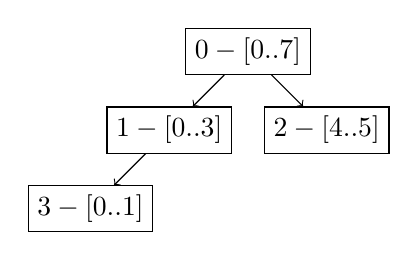
\begin{tikzpicture}
		\node[draw] (root) at (0,0) {$0-[0..7]$};
		
		\node[draw] (1) at (-1,-1) {$1-[0..3]$};
		\node[draw] (2) at (1,-1) {$2-[4..5]$};
		
		\node[draw] (1-1) at (-2, -2) {$3-[0..1]$};
		
		\draw[->] (root) -- (1);
		\draw[->] (root) -- (2);
		
		\draw[->] (1) -- (1-1);
	\end{tikzpicture}
\end{figure}
